% Titre de la premiere partie
\section{Gestion des TP, nouveau protocole}

%%%%%%%%%%%%%%%%%%%%%%%%%%%%%%%%%%%%%%%%%%%%%%%%
%%%%%%%%%%%%%%%%%%%%%%%%%%%%%%%%%%%%%%%%%%%%%%%%
\begin{frame}
	\frametitle{Gestion des TP}
	\framesubtitle{Organisation après GitHub}

	\begin{itemize}[<+->]
		\item	 Dossier de chaque TP distribué via GitHub depuis n'importe où (souvent la maison), le tout pouvant être préparé à l'avance facilement.

		\item  Travail des élèves sur les ordis du lycée ou leur propre ordi en ayant toujours la dernière version à jour (à condition d'avoir pensé à «pousser» leurs derniers commits)

		\item Ramassage des dossiers des élèves de n'importe où (et à n'importe quelle heure) avec possibilité d'imposer une deadline indépendante de l'aspect matériel (on prend le dernier commit avant la deadline, sans compter les suivants).

		\resizebox{\linewidth}{!}{\texttt{git checkout `git rev-list -n 1 --before="2018-09-15 13:37" master`}}

	\end{itemize}

\end{frame}


%%%%%%%%%%%%%%%%%%%%%%%%%%%%%%%%%%%%%%%%%%%%%%%%
%%%%%%%%%%%%%%%%%%%%%%%%%%%%%%%%%%%%%%%%%%%%%%%%
\begin{frame}
	\frametitle{Gestion des TP}
	\framesubtitle{Avantages élèves}

	\begin{itemize}[<+->]
		\item Sauvegarde et archivage automatique du travail des élèves.

		\item Possibilité de poser des questions lors des commits.

		\visible<2-> {
		\begin{center}
				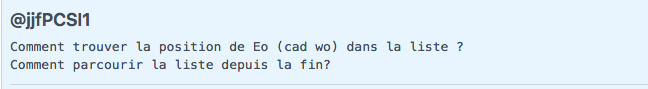
\includegraphics[width=0.8\linewidth]{figures/github_questions_commit.png}
		\end{center}
		}

		\item Feedback possible depuis n'importe où directement dans le code des commits des élèves.

		\visible<3-> {
			\begin{center}
					
\includegraphics[width=0.8\linewidth]{figures/github_commentaires_commit.png}
			\end{center}
		}

	\end{itemize}

\end{frame}

%%%%%%%%%%%%%%%%%%%%%%%%%%%%%%%%%%%%%%%%%%%%%%%%
%%%%%%%%%%%%%%%%%%%%%%%%%%%%%%%%%%%%%%%%%%%%%%%%
\begin{frame}
	\frametitle{Gestion des TP}
	\framesubtitle{Avantages élèves}

	\begin{center}
		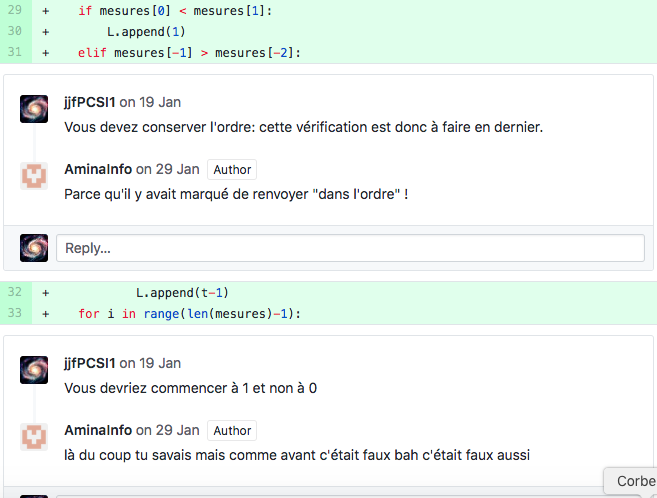
\includegraphics[width=0.8\linewidth]{figures/TP_note_info.png}
	\end{center}

\end{frame}

%%%%%%%%%%%%%%%%%%%%%%%%%%%%%%%%%%%%%%%%%%%%%%%%
%%%%%%%%%%%%%%%%%%%%%%%%%%%%%%%%%%%%%%%%%%%%%%%%
\begin{frame}
	\frametitle{Gestion des TP}
	\framesubtitle{Avantages profs}

	\begin{itemize}[<+->]
		\item Suivi facilité du travail des élèves durant les TP (et au-dehors)

		\item Conseils localisés et personnalisés

		\item Accès direct au code pour identifier les problèmes

		\item Détermination facilitée des fraudeurs potentiels

		\item Gestion entière scriptée, moins de manipulations «manuelles» nécessaires

	\end{itemize}

\end{frame}
